\chapter{Modèles d'évaluation d'options}
\label{sec:modeles}

\section{Le modèle de Black-Scholes}
\subsection{Fondements et hypothèses}

Le modèle de Black-Scholes-Merton, développé en 1973, constitue une révolution dans la théorie financière et représente la pierre angulaire de l'évaluation moderne des options. Il propose une solution analytique élégante pour le prix d'une option européenne, sous l'hypothèse que l'actif sous-jacent suit un \textbf{mouvement brownien géométrique}. Ce modèle repose sur plusieurs hypothèses simplificatrices :

\begin{itemize}
	\item Marché \textbf{sans friction} : absence de frais de transaction et d'impôts,
	\item Respect du principe d'\textbf{absence d'opportunité d'arbitrage},
	\item Possibilité d'effectuer des \textbf{ventes à découvert} sans restriction,
	\item \textbf{Taux d'intérêt} sans risque $r$ constant et connu,
	\item Absence de \textbf{dividendes} pendant la durée de vie de l'option,
	\item \textbf{Volatilité} $\sigma$ du sous-jacent constante,
	\item Prix de l'actif suivant une distribution \textbf{log-normale}.
\end{itemize}

Bien que ces hypothèses soient restrictives, le modèle offre un cadre théorique puissant qui sert de base à de nombreuses extensions.

\subsection{Formulation mathématique}

Dans le cadre de Black-Scholes, le prix du sous-jacent $S_t$ suit un mouvement brownien géométrique. Sous la probabilité historique $\mathbb{P}$, la dynamique de $S_t$ est donnée par :

\begin{equation}
	dS_t = \mu S_t dt + \sigma S_t dB_t,
\end{equation}

où :
\begin{itemize}
	\item $S_t$ est le prix de l'actif à l'instant $t$,
	\item $B_t$ est un mouvement brownien standard,
	\item $\mu$ est le taux de drift,
	\item $\sigma$ est la volatilité constante.
\end{itemize}

En appliquant la formule d'Itô, on obtient la solution explicite :

\begin{equation}
	S_t = S_0 \exp\left( \sigma B_t + \left( \mu - \frac{1}{2} \sigma^2 \right) t \right).
\end{equation}

Ainsi, $\ln S_t$ suit une loi normale de moyenne $\ln S_0 + \left( \mu - \frac{1}{2}\sigma^2 \right)t$ et de variance $\sigma^2 t$.

\subsection{Équation aux dérivées partielles et solution analytique}

Le modèle repose sur la construction d'un portefeuille autofinancé composé d'une position $\Delta$ dans l'actif et d'une position en actif sans risque. En appliquant la formule d'Itô et en neutralisant le risque, on obtient l'équation de Black-Scholes :

\begin{equation}
	\frac{\partial C}{\partial t} + \frac{1}{2}\sigma^2 S^2 \frac{\partial^2 C}{\partial S^2} + rS \frac{\partial C}{\partial S} - rC = 0,
\end{equation}

avec la condition terminale pour un call :

\begin{equation}
	C(T,S) = \max(S-K,0).
\end{equation}

\subsection{Formules fermées de valorisation}

La solution analytique donne le prix d'un call européen :

\begin{equation}
	C_{BS}(S_0,K,T,r,\sigma) = S_0 N(d_1) - Ke^{-rT} N(d_2),
\end{equation}

avec :

\begin{equation}
	d_1 = \frac{\ln(S_0/K) + (r + \frac{1}{2}\sigma^2)T}{\sigma \sqrt{T}}, \quad d_2 = d_1 - \sigma\sqrt{T},
\end{equation}

où $N(\cdot)$ désigne la fonction de répartition de la loi normale centrée réduite.

Le prix d'un put européen est :

\begin{equation}
	P_{BS}(S_0,K,T,r,\sigma) = Ke^{-rT} N(-d_2) - S_0 N(-d_1).
\end{equation}

Ces formules satisfont la relation de parité call-put :

\begin{equation}
	C_{BS} - P_{BS} = S_0 - Ke^{-rT}.
\end{equation}

\subsection{Volatilité implicite}

La \textbf{volatilité implicite} (VI) est la volatilité qui, insérée dans la formule de Black-Scholes, reproduit le prix observé du marché :

\begin{equation}
	C_{BS}(S_0, K, T, r, \sigma) = C_{obs}.
\end{equation}

La recherche de $\sigma$ est réalisée numériquement, notamment via la méthode de Newton-Raphson.

La volatilité implicite constitue un indicateur clé des anticipations du marché.

\subsection{Approche par simulation Monte Carlo}
\label{subsec:bs_monte_carlo}

\subsubsection{Principes de la méthode Monte Carlo}

La méthode Monte Carlo repose sur la simulation de nombreux chemins du prix du sous-jacent pour approximer la valeur de l'option. Le prix est estimé par :

\begin{equation}
	V_0 \approx e^{-rT} \frac{1}{N} \sum_{i=1}^{N} h(S_T^{(i)}),
\end{equation}

où $h(S_T^{(i)})$ est le payoff simulé et $N$ est le nombre de simulations.

\subsubsection{Discrétisation d'Euler-Maruyama pour Black-Scholes}

Sous la mesure risque-neutre, la dynamique est :

\begin{equation}
	dS_t = rS_t dt + \sigma S_t dB_t.
\end{equation}

En discrétisant par pas de temps $\Delta t = T/M$, on obtient :

\begin{equation}
	S_{t_{j+1}} = S_{t_j} + rS_{t_j}\Delta t + \sigma S_{t_j}\sqrt{\Delta t} Z_j,
\end{equation}

où $Z_j \sim \mathcal{N}(0,1)$.

\begin{algorithm}[H]
	\caption{Pricing d'option européenne par Monte Carlo avec schéma d'Euler-Maruyama}
	\begin{algorithmic}[1]
		\State \textbf{Entrées} : $S_0$, $K$, $r$, $\sigma$, $T$, $N$ (simulations), $M$ (pas de temps)
		\State \textbf{Initialisation} : $\Delta t = T/M$, somme\_payoffs = 0
		\For{$i = 1$ to $N$}
		\State $S \gets S_0$
		\For{$j = 1$ to $M$}
		\State Générer $Z \sim \mathcal{N}(0,1)$
		\State $S \gets S + rS\Delta t + \sigma S\sqrt{\Delta t}Z$
		\EndFor
		\State Calculer le payoff
		\State somme\_payoffs $\gets$ somme\_payoffs + payoff
		\EndFor
		\State \textbf{Retour} : $e^{-rT} \times$ somme\_payoffs $/N$
	\end{algorithmic}
\end{algorithm}

\subsection{Limites du modèle et phénomènes de marché}

\subsubsection{Problème de volatilité constante}

La volatilité n'est pas constante en pratique ; elle dépend du strike et de la maturité, formant des \textbf{smiles} et \textbf{skews} de volatilité.

\subsubsection{Caractéristiques empiriques des rendements}

Les rendements observés présentent des \textbf{queues épaisses} et de l'\textbf{asymétrie}, contrairement à l'hypothèse de normalité du modèle.

\subsubsection{Frictions de marché}

En réalité, il existe des coûts de transaction, des restrictions de vente à découvert et des taux d'intérêt variables.

\begin{figure}[H]
	\centering
	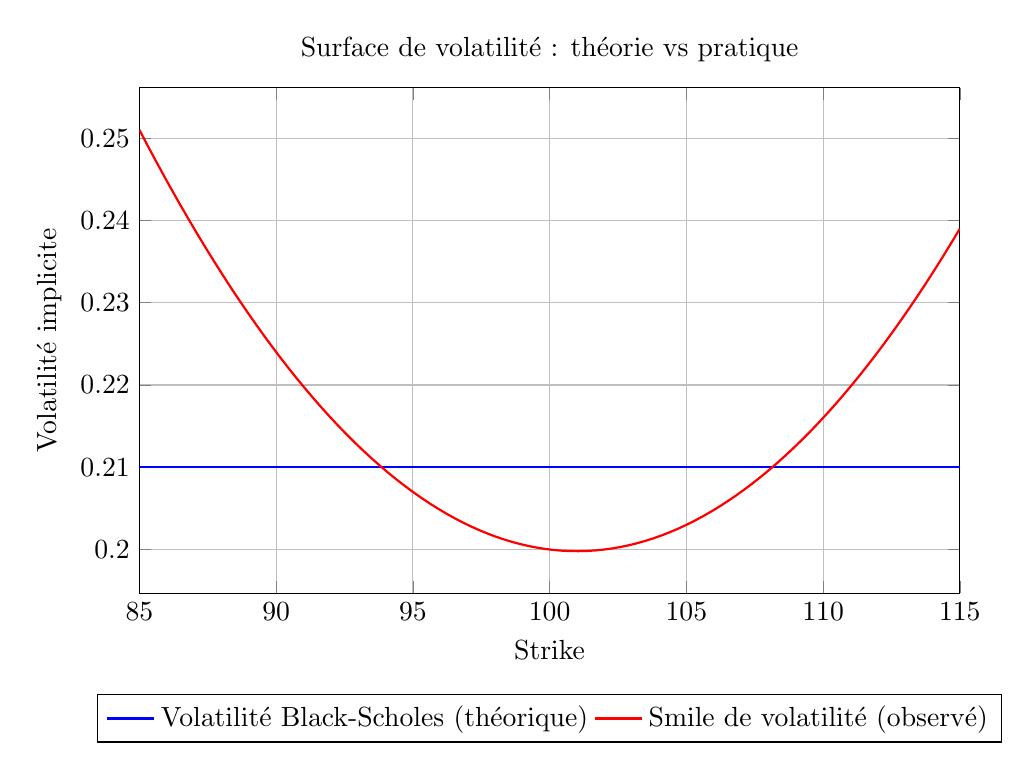
\begin{tikzpicture}
		\begin{axis}[
			width=12cm,
			height=8cm,
			xmin=85, xmax=115,
			xlabel={Strike},
			ylabel={Volatilité implicite},
			grid=both,
			legend style={at={(0.5,-0.2)},anchor=north,legend columns=2},
			title={Surface de volatilité : théorie vs pratique}
			]
			
			\addplot[
			domain=85:115,
			samples=100,
			thick,
			blue
			]
			{0.21};
			\addlegendentry{Volatilité Black-Scholes (théorique)}
			
			\addplot[
			domain=85:115,
			samples=100,
			thick,
			red
			]
			{0.2 + 0.0002*(x-100)^2 - 0.0004*(x-100)};
			\addlegendentry{Smile de volatilité (observé)}
		\end{axis}
	\end{tikzpicture}
	\caption{Contraste entre la volatilité constante de Black-Scholes et le smile observé en pratique.}
	\label{fig:volatility_smile}
\end{figure}

Ces limitations motivent l'étude de modèles plus réalistes, notamment le modèle de Heston que nous aborderons au prochain chapitre.

%%%%%%%%%%%%%%%%%%%%%%%%%%%%%%%%%%%%%%%%%%%%%%%%%%%%%
%%%%%%%%%%%%%%%%%%%  Heston  %%%%%%%%%%%%%%%%%%%%%%%%
%%%%%%%%%%%%%%%%%%%%%%%%%%%%%%%%%%%%%%%%%%%%%%%%%%%%%

\section{Le modèle de Heston}

Le modèle de Heston, introduit par Steven Heston en 1993, constitue une avancée majeure dans la modélisation des options financières. Contrairement au modèle de Black-Scholes qui suppose une volatilité constante, Heston propose un cadre où la volatilité elle-même suit un processus stochastique. Cette approche permet de mieux refléter les réalités observées sur les marchés financiers, notamment les phénomènes de smile et de skew de volatilité.

\subsection{Dynamique du modèle}

Soit $S_t$ le prix de l’actif sous-jacent à l’instant $t$ et $v_t$ sa variance instantanée ($v_t = \sigma_t^2$). Sous la mesure risque-neutre $\mathbb{Q}$, la dynamique du modèle de Heston est donnée par :

\begin{equation}
	\begin{cases}
		dS_t = r S_t dt + \sqrt{v_t} S_t dW_t^{(1)} \\
		dv_t = \kappa(\theta - v_t)dt + \sigma \sqrt{v_t} dW_t^{(2)} \\
		dW_t^{(1)} dW_t^{(2)} = \rho dt
	\end{cases}
\end{equation}

où :
\begin{itemize}
	\item $r$ est le taux d'intérêt sans risque,
	\item $W_t^{(1)}$ et $W_t^{(2)}$ sont deux mouvements browniens corrélés avec coefficient $\rho$,
	\item $\kappa$ est la vitesse de retour vers la moyenne,
	\item $\theta$ est la variance à long terme,
	\item $\sigma$ est la volatilité de la variance (vol-of-vol).
\end{itemize}

\subsection{Interprétation des paramètres}

Le modèle de Heston comporte cinq paramètres principaux, chacun ayant une interprétation financière :

\subsubsection{Volatilité initiale ($v_0$)}
Il s'agit de la valeur initiale de la variance instantanée. Elle représente la perception immédiate de la volatilité du marché.

\subsubsection{Vitesse de retour à la moyenne ($\kappa$)}
Le paramètre $\kappa$ contrôle la rapidité avec laquelle $v_t$ revient vers le niveau moyen $\theta$ après un choc.

\subsubsection{Niveau moyen de variance à long terme ($\theta$)}
Ce paramètre indique la moyenne à long terme autour de laquelle la variance $v_t$ fluctue.

\subsubsection{Volatilité de la volatilité ($\sigma$)}
La vol-of-vol mesure l'ampleur des variations aléatoires de la variance $v_t$.

\subsubsection{Corrélation ($\rho$)}
$\rho$ est la corrélation instantanée entre les variations du prix du sous-jacent et celles de sa variance. En pratique, sur les marchés actions, $\rho$ est souvent négatif (effet de levier).

\subsection{Conditions de Feller et contraintes de positivité}

\subsubsection{Condition de Feller}
La condition de Feller garantit la positivité de $v_t$ :

\begin{equation}
	2\kappa\theta > \sigma^2
\end{equation}

Si elle est satisfaite, le processus de variance évite d'atteindre zéro, ce qui assure la stabilité du modèle.

\subsubsection{Contraintes sur les paramètres}
Pour garantir le réalisme du modèle, on impose :

\begin{align*}
	\kappa &> 0 \quad \text{(vitesse de retour positive)} \\
	\theta &> 0 \quad \text{(niveau moyen positif)} \\
	\sigma &> 0 \quad \text{(volatilité positive)} \\
	v_0 &> 0 \quad \text{(variance initiale positive)}
\end{align*}

\subsection{Équation aux dérivées partielles de Heston}

En utilisant une approche similaire à celle de Black-Scholes mais en prenant en compte la stochastique de la variance, on obtient l'EDP suivante :

\begin{equation}
	\frac{\partial U}{\partial t} + \frac{1}{2} v S^2 \frac{\partial^2 U}{\partial S^2} + \rho \sigma v S \frac{\partial^2 U}{\partial v \partial S} + \frac{1}{2} \sigma^2 v \frac{\partial^2 U}{\partial v^2} + rS \frac{\partial U}{\partial S} + (\kappa(\theta - v) - \lambda) \frac{\partial U}{\partial v} - rU = 0
\end{equation}

où $\lambda$ représente la prime de risque de volatilité.

\subsection{Solution semi-analytique par transformée de Fourier}

Heston propose une solution semi-analytique basée sur la transformée de Fourier. Le prix d'un call européen est exprimé comme :

\begin{equation}
	C(S_0, K, T) = S_0 P_1 - Ke^{-rT} P_2
\end{equation}

où $P_1$ et $P_2$ sont calculés par intégration de la fonction caractéristique :

\begin{equation}
	P_j = \frac{1}{2} + \frac{1}{\pi} \int_0^\infty \text{Re} \left( \frac{e^{-i\phi\ln K} f_j(\phi)}{i\phi} \right) d\phi, \quad j=1,2
\end{equation}

La fonction caractéristique $f_j(\phi)$ est donnée par :

\begin{equation}
	f_j(\phi) = \exp\left( i\phi x + C_j(\tau, \phi) + D_j(\tau, \phi) v_0 \right)
\end{equation}

avec :

\begin{align}
	d_j &= \sqrt{(\rho \sigma i\phi - b_j)^2 - \sigma^2 (2u_j i\phi - \phi^2)} \\
	g_j &= \frac{b_j - \rho\sigma i\phi + d_j}{b_j - \rho\sigma i\phi - d_j} \\
	C_j(\tau, \phi) &= ri\phi\tau + \frac{a}{\sigma^2}\left[ (b_j - \rho\sigma i\phi + d_j)\tau - 2\ln\left( \frac{1 - g_j e^{d_j\tau}}{1 - g_j} \right) \right] \\
	D_j(\tau, \phi) &= \frac{b_j - \rho\sigma i\phi + d_j}{\sigma^2} \left( \frac{1 - e^{d_j\tau}}{1 - g_j e^{d_j\tau}} \right)
\end{align}

où :
\[
a = \kappa \theta, \quad \tau = T - t, \quad x = \ln(S_0)
\]
et
\[
u_1 = \frac{1}{2}, \quad b_1 = \kappa + \lambda - \rho \sigma
\]
\[
u_2 = -\frac{1}{2}, \quad b_2 = \kappa + \lambda
\]

\subsection{Méthode de Monte Carlo}

\subsubsection{Principe général}

La méthode de Monte Carlo simule un grand nombre de trajectoires de $(S_t, v_t)$ pour estimer :

\begin{equation}
	C(K) \approx e^{-rT} \frac{1}{N} \sum_{i=1}^{N} \max(S_T^{(i)} - K, 0)
\end{equation}

où $N$ est le nombre de simulations.

\subsubsection{Schéma de discrétisation d'Euler-Maruyama}

Le modèle est discrétisé comme suit :

\begin{equation}
	\begin{aligned}
		v_{t+\Delta t} &= v_t + \kappa(\theta - v_t^+)\Delta t + \sigma\sqrt{v_t^+}\sqrt{\Delta t}Z_v \\
		S_{t+\Delta t} &= S_t \exp\left( \left(r - \frac{v_t^+}{2}\right)\Delta t + \sqrt{v_t^+}\sqrt{\Delta t}Z_S \right)
	\end{aligned}
\end{equation}

avec $Z_S$ et $Z_v$ deux variables normales corrélées :

\[
Z_v = \rho Z_S + \sqrt{1 - \rho^2} Z_\perp
\]

\subsubsection{Traitement des valeurs négatives de variance}

Pour éviter les variances négatives :

\begin{itemize}
	\item \textbf{Full truncation} : $v_t^+ = \max(v_t, 0)$
	\item \textbf{Réflexion} : $v_t^+ = |v_t|$
\end{itemize}

\subsubsection{Réduction de variance : variables antithétiques}

Pour chaque trajectoire basée sur un bruit $Z$, on simule également la trajectoire opposée $-Z$. L'estimateur est donné par :

\[
V = \frac{1}{2}(f(Z) + f(-Z))
\]

Cette méthode améliore la précision en diminuant la variance de l'estimation.

\subsubsection{Avantages et limites}

\begin{itemize}
	\item \textbf{Avantages} : Flexibilité, applicable à divers types d'options.
	\item \textbf{Limites} : Convergence lente ($\mathcal{O}(1/\sqrt{N})$), coûteux en temps de calcul.
\end{itemize}

\section{Conclusion}

Dans ce chapitre, nous avons présenté deux piliers majeurs de la modélisation du prix des options : le modèle de Black-Scholes et son extension naturelle, le modèle de Heston à volatilité stochastique.

%Le modèle de Black-Scholes, bien qu'élégant et fondateur, repose sur des hypothèses simplificatrices telles que la constance de la volatilité, qui se révèlent insuffisantes pour capturer certaines caractéristiques empiriques des marchés financiers, notamment les smiles et skews de volatilité. 

%En réponse à ces limites, le modèle de Heston introduit une dynamique plus réaliste où la volatilité est elle-même gouvernée par un processus stochastique de type CIR, corrélé au prix du sous-jacent. Nous avons détaillé la structure mathématique du modèle de Heston, ses conditions de viabilité (comme la condition de Feller), ainsi que deux approches principales de pricing : la méthode semi-analytique basée sur les fonctions caractéristiques et l'approche par simulations Monte Carlo.

La richesse du modèle de Heston réside dans sa capacité à reproduire de nombreuses observations de marché tout en restant relativement tractable sur le plan computationnel. Ce modèle servira de base aux développements ultérieurs de notre projet, notamment pour la calibration aux données de marché et la comparaison de différentes méthodes numériques de valorisation.

Le prochain chapitre sera dédié à l'étude approfondie de la calibration du modèle de Heston, étape cruciale pour assurer son adéquation avec les données de marché réelles.



